\subsection*{\Large Общая характеристика работы}
\fontsize{14pt}{15pt}\selectfont
\textbf{Актуальность темы.}
Сердечно-сосудистые заболевания являются одной из наиболее острых проблем
современного общества. Во всех странах их количество существенно опережает
остальные в силу ряда социальных причин (экономические изменения, урбанизация и
проч. приводят к изменению образа жизни многих людей) и увеличения влияния
факторов риска (например, уменьшение физической активности), поэтому трудно
переоценить значимость исследований в этой области. В последние годы
наблюдается резкий рост интереса к проблеме сердечно-сосудистых заболеваний,
развиваются новые методики исследования, появляются все более точные
измерительные приборы. Одним из самых эффективных способов лечения таких
заболеваний является протезирование. Каждый год в мире проводится
примерно 250 000 операций восстановлению или замене поврежденных сердечных
клапанов\footnote{
    Yoganathan A.P., He Z.M., Jones S.C.: Fluid mechanics of heart valves.  Annu. Rev.
    Biomed Eng 6:331--362 (2004)
} % replace with new statistics
и ожидается, что в ближайшие годы это значение будет только увеличиваться\footnote{
    Yacoub N, Takkenberg J.: Will heart valve tissue engineering change the world? Nat
    Clin Prac Cardiovas Med. 2:60--1 (2005)
}.
Искусственные сердечные клапаны являются одними из самых сложных биопротезов,
используемых в кардиохирургии. Они позволяют эффективно бороться с
заболеваниями и повреждениями естественных клапанов, но при этом не являются
достаточно долговечными и при их использовании могут проявляться побочные
явления. Например, механические клапаны обладают высокой надежностью и
долговечностью, но могут приводить к сильным деформациям потока, формированию
сгустков кровяных клеток и как следствие - к образованию тромбов. Биологические
клапаны лишены этого недостатка, однако они менее долговечны и их изготовление
достаточно сложная техническая задача, которая до сих пор полностью не решена.
Так как проведение лабораторных и тем более натурных экспериментов является
очень сложной задачей, математическое моделирование работы искусственного
клапана, аналогичного естественному, позволяет получить более глубокое
понимание взаимодействия потока крови и клапана и тем самым найти пути
усовершенствования их конструкции.

Несмотря на актуальность проблемы, исследования в данной области все еще требуют
значительных усилий в силу ряда проблем, которые приводят к существенным трудностям
при постановка задачи и ее численном решении:
\begin{enumerate}
 \item Кровь является неньютоновской жидкостью и имеет сложную структуру
 \item Створки клапана чрезвычайно тонкие, но при этом могут выдерживать
     большие перепады давления
 \item Взаимодействие течения жидкости и гибких створок приводит к сложной
     геометрии исследуемых объектов
\end{enumerate}

%При изучении подобных явлений методами математического моделирования зачастую
%удовлетворительные результаты можно получить с помощью модели вязкой
%несжимаемой жидкости, которая описывается системой дифференциальных уравнений
%Навье-Стокса, выписанных в форме естественных переменных <<скорость-давление>>.
%Помимо этого требуется учесть, что кровь является неоднородной по своей природе
%и состоит из плазмы и форменных элементов (лейкоциты, эритроциты и т.д.), а
%сосуды и клапаны являются гибкими и изменяют форму под воздействием различных
%параметров. Необходимость описывать взаимодействия гибких непроницаемых тканей
%с неоднородной жидкостью приводит к существенным трудностям при постановке
%задачи и ее численном решении, связанными с построением расчетной сетки и ее
%изменением в соотвтетсвии с движением лепестков клапана и деформацией сосуда.

Существует несколько устоявшихся подходов, для того, чтобы избежать эти
трудности, однако полноценной модели, которая бы учитывала все указанные
факторы, на сегодняшний момент не предложено. Все существующие работы в этой
области обычно концентрируются на какой-либо одной из проблем, поэтому
математическое моделирование искусственных сердечных клапанов и дальнейшее развитие
методов вычислительной гидродинамики, применяемых для его численного моделирования,
в настоящее время является актуальной проблемой.

\textbf{Целью} данной работы является разработка технологии решения
нестационарной трехмерной задачи о движении створок искусственного клапана
внутри крупных кровеносных сосудов с учетом неоднородной структуры крови, а
также о движении примеси (форменных элементов) внутри сосуда. Для достижения
этой цели был создан программный комплекс, с помощью которого можно
моделировать работу клапана, деформацию стенок кровеносных сосудов и получать
картины течения внутри них.

Для достижения поставленной цели необходимо решить следующие \textbf{задачи}:
\begin{enumerate}
 \item Разработать и реализовать численные алгоритмы решения систем нестационарных
     уравнений Навье-Стокса, нахождения энергии деформации исходя их гипотезы Эйлера-Бернулли,
     а также взаимодействия течения жидкости и гибких непроницаемых препятствий
     на основе метода погруженной границы
     % гипотеза эйлера-бернулли https://ru.wikipedia.org/wiki/Изгиб_(механика)
 \item Разработать программный комплекс на основе построенных численных алгоритмов
     для расчета течения вязкой несжимаемой неоднородной жидкости в канале
     с гибкими непроницаемыми препятствиями
 \item Провести тестирование разработанного программного комплекса, получить
     результаты расчетов модельных трехмерных задач, сравнив их с существующими
     результатами других авторов
 \item Применить разработанный программный комплекс для численного моделирования
     работы искусственного сердечного клапана и сравнить полученные результаты
     с экспериментальными
 \item Провести численные эксперименты с различными параметрами жидкости и клапана
     и сформировать набор рекомендаций по улучшению характеристик искусственного сердечного клапана.
\end{enumerate}

\textbf{Методы исследования}.
В исследовании применялись методы механики сплошных сред, методы теории
упругости, методы теории разностных схем, методы теории итерационных схем
решения систем алгебраических уравнений.\\

\textbf{Основные результаты, выносимые на~защиту.}
В работе присутствуют результаты, соответствующие трем областям исследования
паспорта специальности 05.13.18 – «Математическое моделирование, численные
методы и комплексы программ» по физико-математическим наукам.

\begin{enumerate}
    \item Численные алгоритмы решения задачи о течении вязкой несжимаемой
        неоднородной жидкости в канале с гибкими непроницаемыми препятствиями при
        заданном перепаде давления, включающая алгоритм взаимодействия жидкости с
        границей, а также способ расчета движения примесей.
    \item Результаты расчетов трехмерных задач о работе искусственного сердечного
        клапана, а также течения вязкой несжимаемой неоднородной жидкости в
        крупных кровеносных сосудах.
\end{enumerate}

\textbf{Научная новизна:}
\begin{enumerate}
 \item Предложена оригинальная технология решения трехмерной задачи о движении
     вязкой несжимаемой неоднородной жидкости в каналах сложной формы с гибкими
     границами.
 \item С помощью созданного программного комплекса впервые были решены
     трехмерные задачи о работе створок клапана <<Юнилайн>>, а также о деформации стенок
     крупных кровеносных сосудов с учетом неоднородной структуры крови.
\end{enumerate}

\textbf{Обоснованность и достоверность} изложенных в работе результатов
обеспечивается использованием полностью консервативных схем для аппроксимации
решаемой дифференциальной задачи, применением сходящихся итерационных методов
для решения систем нелинейных алгебраических уравнений, а также совпадением
полученных результатов методических расчетов с решениями, полученными другими
авторами, и с экспериментальными данными.\\

\textbf{Теоретическая значимость} диссертационной работы обуславливается:
новизной подхода к моделированию работы искусственного сердечного клапана,
позволяет использовать метод погруженной границы для многокомпонентной жидкости;
альтернативным способом дискретизации численной схемы по времени; новизной
результатов численного моделирования работы клапана <<Юнилайн>>.

\textbf{Практическая значимость} исследования определяется
возможностью использования полученных методов и разработанного программного
комплекса для оптимизации структуры искусственных сердечных клапанов, а также
применением созданного комплекса программ при выполнении государственного
задания № 1.630.2014/К <<Моделирование течения с переменной плотностью
и вязкостью при решении прикладных задач>>.\\

\textbf{Представление работы.}
Основные результаты работы докладывались и обсуждались на следующих
конференциях: Международной конференции <<Информационно-вычислительные
технологии и математическое моделирование (ИВТ\&ММ)>>, Россия, Кемерово, 2013
г.; XIII Международной научно-практической конференции <<Информационные
технологии и математическое моделирование>> им. А. Ф. Терпугова, Россия,
Анжеро-Судженск, 2014 г.; Международной научной студенческой конференции,
Россия, Новосибирск, 2015 г.; VIII Международной конференции, посвященной
115-летию со дня рождения академика Михаила Алексеевича Лаврентьева, Россия,
Новосибирск, 2015 г.; International Conference <<Computational and
Informational Technologies in Science, Engineering and Education>>, Казахстан,
Алматы, 2015 г.; III International Conference in memory of V.I.Zubov
<<Stability and Control Processes>>, Россия, Санкт-Петербург, 2015 г.; Шестая
научно-практическая сессия молодых ученых Кузбасса «Наука-практике» в области
сердечно-сосудистых заболеваний, г. Кемерово, 2016; Международная конференция
<<Математическое моделирование и высокопроизводительные вычисления в
биоинформатике, биомедицине и биотехнологии>>, г. Новосибирск, 2016;

Также, результаты работы докладывались на семинаре <<Математические модели.
Методы решения>>, Кемерово (под рук. проф. Ю.Н. Захарова).

\textbf{Публикации.} Основные результаты по теме диссертации изложены в 7
печатных изданиях, 1 из которых изданы в журналах, рекомендованных ВАК, 2 -- в
прочих изданиях, 4 --- в тезисах докладов.

\textbf{Личный вклад.} Результаты работы базируются на ряде фундаментальных
исследований, которые относятся к методу погруженной границы\footnote{ Peskin,
    C. S.: The immersed boundary method. Acta Numerica 11, 479–517 (2002).  },
который позволяет расчитывать движение сколь угодно тонких лепестков под
давлением жидкости, а также подходам к решению задач о течении вязкой
несжимаемой неоднородной жидкости под воздействием перепада давления\footnote{
    Gummel E.E., Milosevic H., Ragulin V.V., Zakharov Y.N., Zimin A.I.: Motion
    of viscous inhomogeneous incompressible fluid of variable viscosity.
    Zbornik radova konferencije MIT 2013, Beograd, 267-274 (2014) }. В
настоящей работе автор объединил эти подходы и реализовал программный комплекс
для численного решения задачи о движении створок сердечного клапана, который
использует эти методы. Помимо этого автором проведены расчеты динамики створок
клапана <<Юнилайн>>, а также деформации стенок крупных кровеносных сосудов с
учетом неоднородной структуры крови.

\textbf{Объем и структура работы.}
Диссертация состоит из введения, трех глав, заключения, списка цитируемой
литературы из {\todo N} наименований, {\todo M} таблиц и {\todo K} рисунков.
Общий объем диссертации составляет {\todo L} страниц.

%\newpage
\subsection*{\Large Содержание работы}
Во \textbf{введении} формулируются цели диссертационной работы,
обосновывается актуальность решаемых задач, приводится обзор научной
литературы по изучаемой тематике, излагается краткое содержание работы.

\textbf{Первая глава} состоит из четырех параграфов и посвящена описанию
предметной области, основных биологических особенностей и структуры кровеносной
системы и сердечных клапанов человека. Вводятся основные понятия, описывается
используемая математическая модель, применяемые методы решения, разностные
схемы, а также используемый программный комплекс.

В \textbf{параграфе 1.1} дается описание основных понятий и терминов из
биологии и медицины, структурные особенности клапанов сердца и кровеносной
системы, которые необходимо учитывать при моделировании.

В \textbf{параграфе 1.2} рассматривается система дифференциальных уравнений
Навье-Стокса, которая моделирует нестационарную задачу о течении вязкой
неоднородной несжимаемой жидкости под воздействием перепада давления:
\begin{gather}
    \label{eq:navier_stokes:motion}
    \frac{\partial \vec{u}}{\partial t} + (\vec{u} \cdot \nabla) \vec{u} = - \frac{1}{\rho} \nabla p + \nabla \sigma + \vec{f}\\
    \label{eq:navier_stokes:continuity}
    \frac{\partial \rho}{\partial t} + \nabla \cdot (\rho \vec{u}) = 0
\end{gather}
с начальными и краевыми условиями:
\begin{gather}
    \label{eq:navier_stokes:velocity_conditions}
    \vec{u}(\bar{x}, 0) = \vec{u}_0 \qquad \vec{u}|_{\Gamma_1, \Gamma_4} = \vec{u}_b \qquad u_{\Gamma_2, \Gamma3} = 0\\
    \label{eq:navier_stokes:pressure_conditions}
    p_{\Gamma_2} = p_{in} \qquad p_{\Gamma_3} = p_{out}
\end{gather}
где $\bar{x}=(x,y,z) \in \Omega$, $\vec{u}=(u,v,w)$ - вектор скорости,
$\vec{u}_b$ - скорость, с которой двигаются стенки сосуда и створки клапана при
деформации, $\rho=\rho(\bar{x}, t)$ - плотность, $p=p(\bar{x}, t)$ - давление,
$\sigma = \mu (\nabla \vec{u} + (\nabla \vec{u})^T)$ - вязкий тензор
напряжений, $\mu = \mu(\bar{x}, t)$ - вязкость жидкости, $\vec{f} =
\vec{f}(\bar{x}, t)$ - вектор массовых сил, который в дальнейшем используется
для определения формы сосуда и створок клапана.

Область $\Omega$ изображена на рис. \ref{img:boundaries} и представляет собой
сосуд с границей $\Gamma = \Gamma_1 \cup \Gamma_2 \cup \Gamma_3 \cup \Gamma_4$,
где $\Gamma_1$ - стенка кровеносного сосуда, $\Gamma_2$ и $\Gamma_3$ -  области
втекания и вытекания, $\Gamma_4$ - створки клапана.

Одна из сложностей при численном решении подобных задач заключается в
отсутствии одного компонента вектора скорости на границах $\Gamma_2$,
$\Gamma_3$. Для того, чтобы решить эту проблему, в данной работе на указанных
границах используется оригинальные уравнения (\ref{eq:navier_stokes:motion}) -
(\ref{eq:navier_stokes:pressure_conditions}), что позволяет определить
недостающие компоненты.

\begin{figure}[h]
  \center
  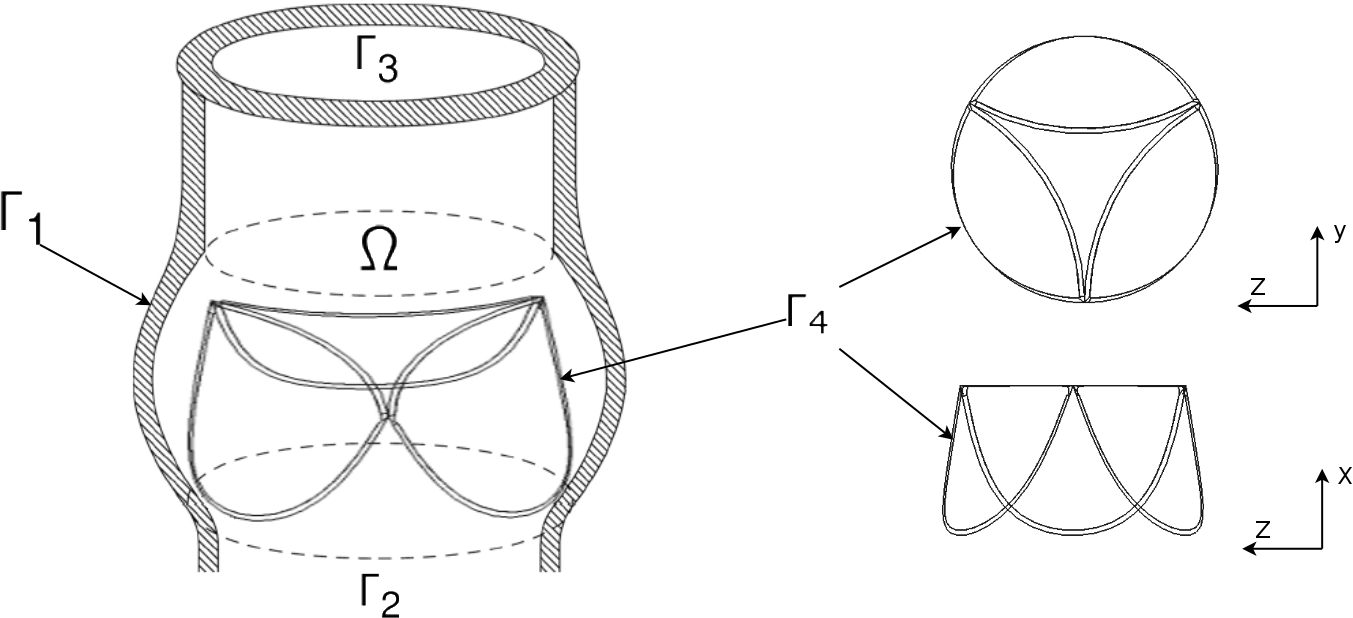
\includegraphics [width=0.9\textwidth] {aorta_valve_scheme.png}
  \caption{Изображение границ расчетной области}
  \label{img:boundaries}
\end{figure}

В этом же параграфе рассматриваются уравнения, используемые для
моделирования изменения плотности и вязкости жидкости, а также концентрации
примесей.  Плотность $\rho$ и вязкость $\mu$ определяются следующими
соотношениями:
\begin{gather}
    \label{eq:viscosity}
    \mu = c (\mu_2 - \mu_1) + \mu_1\\
    \label{eq:density}
    \rho = c (\rho_2 - \rho_1) + \rho_1
\end{gather}
где $\rho_1$, $\mu_1$ - плотность и вязкость жидкости (плазмы), $\rho_2$,
$\mu_2$ - плотность и вязкость примеси (форменных элементов), $c$ -
концентрация примеси.  Концентрация $c=c(\bar{x}, t)$, $c \in [0, 1]$ примеси
определяется как решение уравнения:
\begin{gather}
    \label{eq:convection}
    \frac{\partial c}{\partial t} + \vec{u} \cdot \nabla c = 0
\end{gather}

с начальными условиями и краевыми условиями на границе втекания:
\begin{gather}
    \label{eq:convection:conditions}
    c(\bar{x}, 0) = c_0(\bar{x}), \bar{x} \in \Omega \qquad c(\bar{x}, t)|_{\Gamma_2} = c_s(\bar{x}, t)
\end{gather}

Помимо этого рассматривается задача моделирования движения стенок
сосуда и лепестков клапана, а также их взаимодействия с течением жидкости.
Деформация $\Gamma_1 \cup \Gamma_4$ под воздействием давления жидкости
определяется силами, которые возвращают их в равновесное состояние. При этом
створки клапана $\Gamma_4$ могут деформироваться гораздо сильнее, чем стенки
сосуда $\Gamma_1$. Для описания сил, возникающих при деформации клапана, мы
используем следующую формулу:
\begin{gather}
    \label{eq:boundary_force}
    F = \frac{\partial}{\partial s} (T \tau) + \frac{\partial^2}{\partial s^2} (E \cdot I \frac{\partial^2}{\partial s^2} X)
\end{gather}
где $\bar{q}=(q, r, s) \in \Gamma_4$, $X(\bar{q})$ - функция, описывающая
поверхность створок клапана в момент времени $t$, координаты $q, r, s$ мы
выбираем так, чтобы поверхность $X$ была представлена набором параметрических
линий $s \rightarrow X(q^0, r^0, s)$, $T$ -напряжение, возникающее при
растяжении вдоль $s$, $\tau$ - единичный вектор, касательный к поверхности
клапана, $E$ - модуль Юнга, $I$ - момент инерции поперечного сечения. Формула
(\ref{eq:boundary_force}) позволяет учитывать любые изменения формы створок
клапана.  Для вычисления сил, возникающих при изменении формы сосуда, мы
используем другую формулу, которая позволяет учитывать только небольшие
изменения формы:
\begin{gather}
    \label{eq:boundary_force_simple}
    F = k \|X - X_0\|
\end{gather}
где $\bar{q} = (q, r, s, t) \in \Gamma_1$, $X(\bar{q}, t)$, $X_0(\bar{q}, 0)$ -
функции, которые описывают поверхность сосуда в момент времени $t$ и в
начальный момент времени, $k$ - коэффициент жесткости.

Для того, чтобы учитывать взаимодействие стенок сосуда и створок клапана с
течением жидкости, необходимо на основе силы $F$ вычислить поле внешних сил $f$
в уравнении Навье-Стокса и исходя из поля скоростей жидкости $\vec{u}(\bar{x},
t)$ определить текущую форму $X(bar{q}, t)$ сосуда и клапана. Это делается с
помощью следующих уравнений:
\begin{gather}
    \label{eq:interaction:velocity}
    \frac{\partial X}{\partial t}(\bar{q}, t) = \int_{\Omega} \vec{u}(\bar{x}, t) \cdot \delta (x - X(\bar{q}, t))\; dx\; dy\; dz\\
    \label{eq:interaction:force}
    \vec{f}(\bar{x}, t) = \int_{\Gamma} \vec{F}(\bar{q}, t) \cdot \delta (x - X(\bar{q}, t))\; dq\; dr\; ds
\end{gather}
где $\bar{q} = (q, r, s) \in \Gamma$ - точка поверхности сосуда или клапана, $X
= X(\bar{q}, t)$ - функция, описывающая поверхность сосуда и клапана в момент
времени $t$, $F = F(\bar{q}, t)$ - сила сопротивления деформации в данной
точке, $\vec{u}(\bar{x}, t)$ - вектор скорости течения, $\vec{f}(\bar{x}, t)$ -
вектор массовых сил, $\delta$ - дельта-функция Дирака.

В \textbf{параграфе 1.3} рассматриваются методы, используемые для решения
поставленной задачи, приводятся известные теоремы о существовании и
единственности решения.

Для решения поставленных краевых задач используется метод погруженной границы,
который основывается на том, что при обтекании какого-либо тела жидкостью, она
испытывает влияние силы, действующие по направлению нормали к поверхности тела,
а также сдвиговые силы, если на границе тела поставлено условие прилипания.
Поверхность тела также испытывает влияние тех же сил с противоположным знаком.
Поэтому моделирование обтекания тела возможно с помощью формирования
соответствующего поля внешних массовых сил.  В результате поставленная задача
разбивается на несколько более мелких. Вводятся новые области $\tilde{\Omega}$,
которая представляет собой параллепипед, содержащий в себе $\Omega$, а также
$\Gamma$ с лагранжевой системой координат, которая соотносится со стенками
сосуда и лепестками клапана.  Помимо этого вводятся две сетки
$\tilde{\Omega_h}$ с шагами $h_x$, $h_y$, $h_z$, и $\tilde{\Gamma_h}$, с шагами
$h_q$, $h_r$, $h_s$. $\tilde{\Omega_h}$ является обычной декартовой сеткой и
предназначена для расчет течения жидкости, $\tilde{\Gamma_h}$ - для расчета
деформации стенок сосуда и клапана.

В параграфе описывается численное решение задачи о течении вязкой
несжимаемой жидкости с помощью схемы расщепления по физическим факторам:
\begin{gather}
    \label{eq:splitting:intermediate_velocity}
    \frac{u^* - u^n}{\triangle t} = - (u^n \cdot \nabla) u^* - \frac{1}{\rho} \nabla \sigma + f^n\\
    \label{eq:splitting:poisson}
    \rho \triangle p^{n+1} - \nabla \rho \cdot p^{n+1} = \frac{\rho^2 \nabla u^*}{\triangle t}\\
    \label{eq:splitting:velocity}
    \frac{u^{n+1} - u^*}{\triangle t} = - \frac{1}{\rho} \triangle p^{n+1}
\end{gather}

Численная реализация этой схемы состоит из трех шагов. Вначале вычисляется
промежуточное поле скоростей $u^{*}$, для этого методом стабилизирующей
поправки решается уравнение (\ref{eq:splitting:intermediate_velocity}). После
этого с помощью метода бисопряженных градиентов из уравнения
(\ref{eq:splitting:poisson}) определяется новое поле давления и по формулам
(\ref{eq:splitting:poisson}) расчитывается итоговое поле скоростей.

Помимо этого рассматривается численное решение уравнения переноса
примесей, а также способ расчета вязкости и плотности жидкости.  Для этого
методом стабилизирующей поправки решается следующее уравнение:
\begin{gather}
    \label{eq:numerical_concentration}
    \frac{c^{n+1} - c^{n}}{\triangle t} + u^{n} \cdot \nabla c^{n+1} = 0
\end{gather}
после чего по явным формулам (\ref{eq:viscosity}), (\ref{eq:density})
вычисляются значения $\mu_{n+1}$, $\rho_{n+1}$.

Помимо этого описывается метод численного решения задачи деформации
гибких лепестков клапана, а также взаимодействия "жидкость-клапан".  Деформация
определяется по явным формулам
(\ref{eq:boundary_force}),(\ref{eq:boundary_force_simple}) исходя из формы
сосуда в текущий $X_{n}$ и предыдущий $X_{n-1}$ шаг по времени.  Взаимодействие
"жидкость-клапан" расчитывается с помощью формул
(\ref{eq:interaction:velocity}), (\ref{eq:interaction:force}) в
конечно-разностном виде, где интегралы вычислены с помощью квадратурной формулы
прямоугольников:
\begin{gather}
    \label{eq:numerical_interpolation}
    U_n = \sum_{ijk}u_{ijk} \cdot D(x_{ijk} - x_n) h_{ijk}^3 \\
    \label{eq:numerical_spreading}
    f_{ijk} = \sum_n F_n \cdot D(x_{ijk} - x_n) h^2_n
\end{gather}
где $U_n$, $F_n$ - скорость движения лепестков клапана под воздействием
давления жидкости и сила сопротивления деформации, $u_n$, $f_n$ - скорость
движения жидкости и массовые силы в уравнении (\ref{eq:navier_stokes:motion}),
$D$ - конечно-разностный аналог функции Дирихле, который в данной работе
представлен следующим соотношением:
\begin{gather}
    \label{eq:numerical_dirichlet}
    \begin{cases}
        D(r) = \frac{1}{4h} (1 + cos(\frac{\pi r}{2h})) & |r| < 2h\\
        D(r) = 0 & |r| > 2h\\
    \end{cases}
\end{gather}

В \textbf{параграфе 1.4} дается описание программного комплекса,
предназначеного для моделирования работы створок клапана под воздействием
давления жидкости. Он является модулем для комплекса <<XFlow>> и содержит
библиотеки классов, реализующих описанный выше алгоритм, а также компоненты
пред- и постобработки. Эти компоненты предоставляют возможность использовать
для расчета CAD модели реальных объектов, полученных путем сканирования,
задавать их внутреннюю структуру, т.е.  связи между отдельными узлами, а также
проводить визуализацию и анализ полученных результатов с помощью ParaView и
Matplotlib.

\textbf{Вторая глава} представлена тремя параграфами и посвящена исследованию
задачи течения вязкой несжимаемой неоднородной жидкости в канале с гибкими
стенками, а также решению задачи о развитии аневризмы на стенке кровеносного
сосуда.

В \textbf{параграфе 2.1} представлено решение тестовой безразмерной задачи о течении вязкой
несжимаемой однородной жидкости под воздействием перепада давления $\triangle P = 0.1$ внутри
канала цилиндрической формы длинной $l = 1$, радиусом $r = 0.25$. Жесткость стенок канала $k = 10^{3}$,
что для данной задачи эквивалено жесткой недеформируемой стенке.  На Рис. \ref{img:velocity_profile}
показано сравнение профиля рассчитанной скорости в центре канала с соответствующим аналитическим
решением для шага $0.001$. % разница 6.3\%.
\begin{wrapfigure}{L}{0.5\textwidth}
  \center
  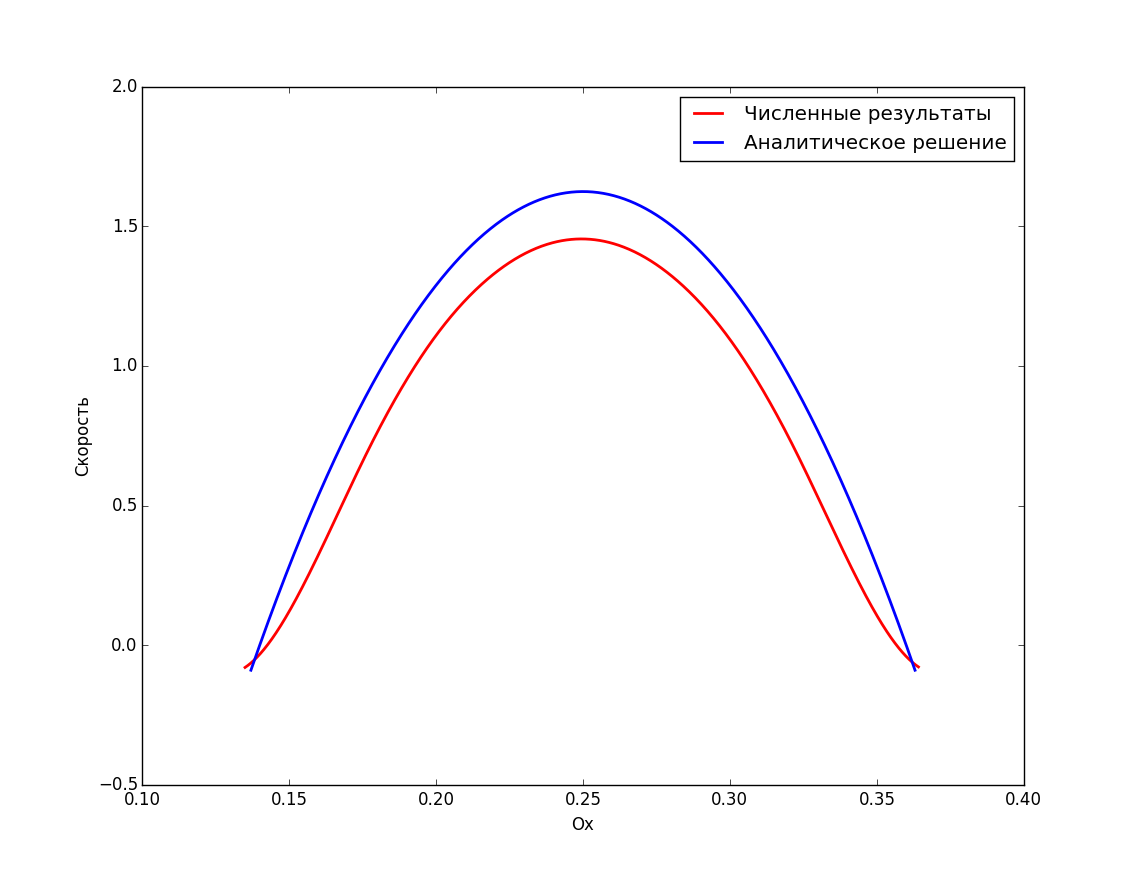
\includegraphics [width=0.4\textwidth] {velocity_profile.png}
  \caption{Сравнение профиля скорости, полученной в расчетах, с аналитическим решением}
  \label{img:velocity_profile}
\end{wrapfigure}

\begin{figure}[H]
  \center
  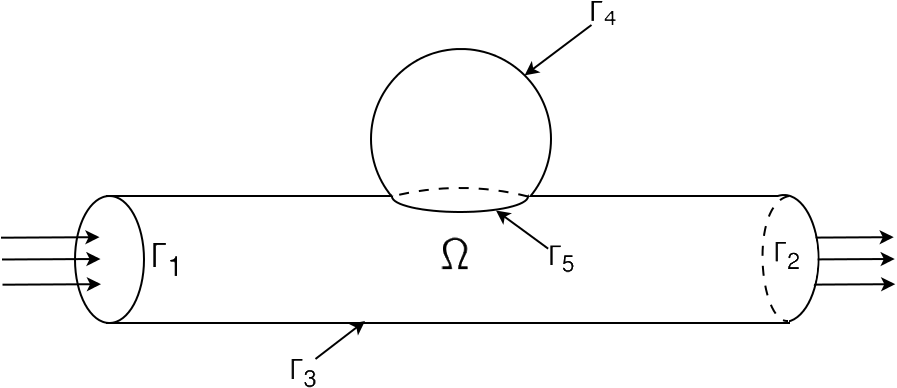
\includegraphics [width=0.9\textwidth] {aneurysm_schema.png}
  \caption{Изображение границ расчетной области}
  \label{img:aneurysm_boundaries}
\end{figure}

В \textbf{параграфе 2.2} описаны результаты решения задачи о моделировании
возникновения аневризмы на стенках кровеносного сосуда.  Постановка задачи
аналогична описанной в \textbf{главе 1}. Т.к. основным объектом исследования является аневризма стенки сосуда,
в задаче отсутствует клапан (см. Рис. \ref{img:aneurysm_boundaries}). На
стенках сосуда выделена область $\Gamma_5$, жесткость которой меньше,
чем жесткотсть остальной части сосуда. Это позволяет моделировать истончение стенки
сосуда и возникновение аневризмы под воздействием давления жидкости.

Были получены результаты для сосудов различных форм и различных параметров текущей жидкости
с целью выяснить, при каких начальных данных возникновение аневризмы неизбежно и какие факторы
наиболее сильно на это влияют.
На Рис. \ref{img:aneurysm_geom3} показана динамика возникновения аневризмы на изгибе сосуда
цилиндрической формы радиуса $r=0.25$ с постоянным перепадом давления $\triangle P=10$.
При данных параметрах возникающая аневризма обладает достаточно симметричной стабильной формой.

\begin{figure}[h]
  \center
  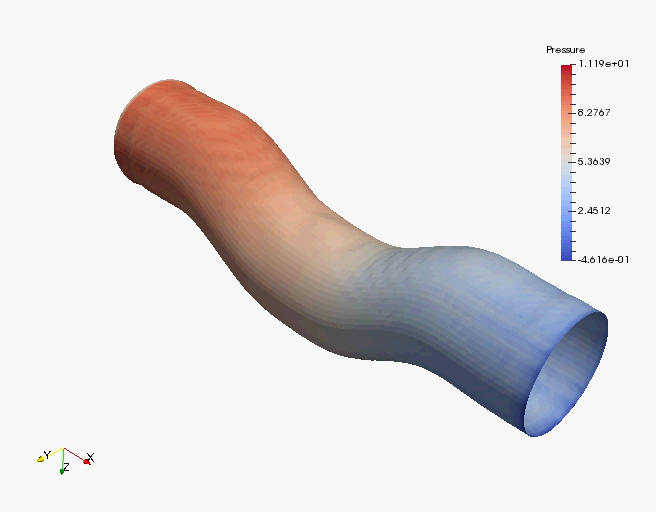
\includegraphics [width=0.45\textwidth] {aneurysm_geom3_0.png}
  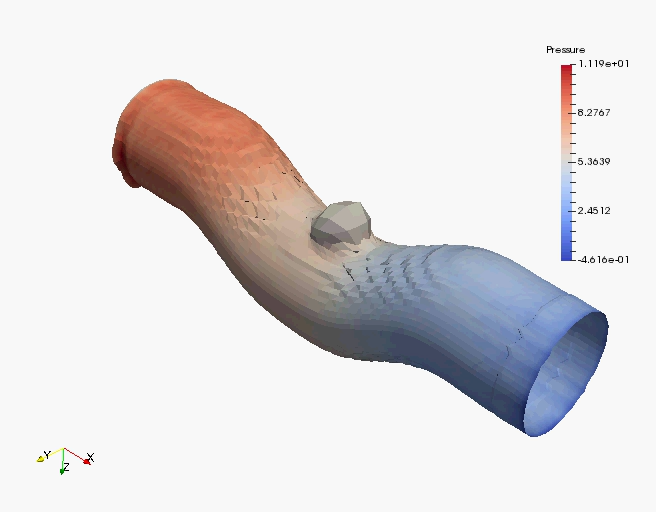
\includegraphics [width=0.45\textwidth] {aneurysm_geom3_2.png}
  \caption{Динамика развития аневризмы стенок изогнутого сосуда}
  \label{img:aneurysm_geom3}
\end{figure}

Расчеты, проведенные для пульсового перепада давления и наличия примеси демонстрируют, что
развитие аневризмы в данных условиях сильнее зависит от начальных данных, т.к. стенка сосуда
не испытывает постоянного давления (см. Рис. \ref{img:aneurysm_geom1}).

\begin{figure}[h]
  \center
  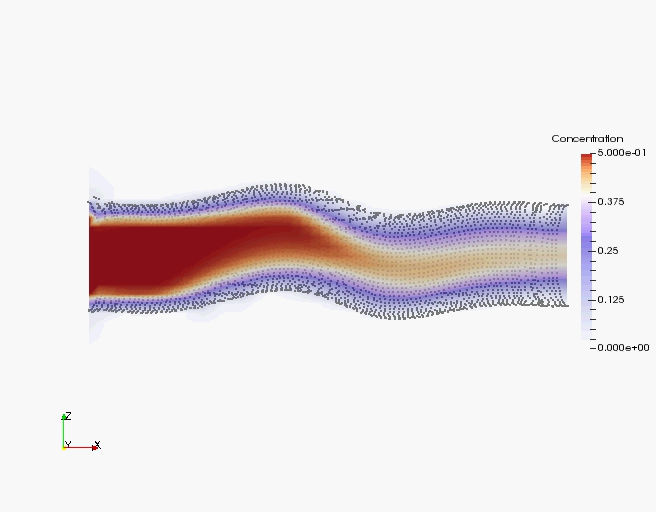
\includegraphics [width=0.45\textwidth] {admixture_geom1_0.png}
  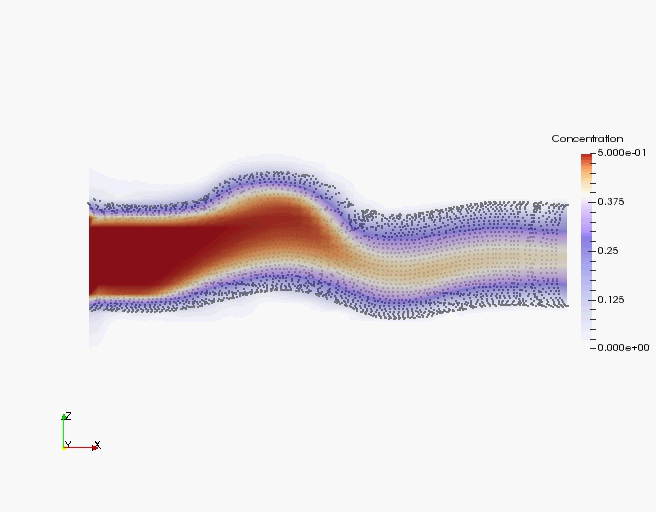
\includegraphics [width=0.45\textwidth] {admixture_geom1_1.png}
  \caption{Динамика развития аневризмы стенок изогнутого сосуда при наличии примеси и пульсового давления}
  \label{img:aneurysm_geom1}
\end{figure}

В \textbf{параграфе 2.3} приведены результаты моделирования движения тробма в сосудах
с разной степенью стеноза. Тромб в расчетах моделируется в виде сгустка примеси высокой
плотности и вязкости, который движется в сосуде. В расчетах получилось обнаружить ситуацию,
когда тромб забивает сосуд на протяжении длительного времени, пока не будет размыт набегающим
потоком жидкости. На Рис. \ref{img:strong_stenosis} показан один из таких расчетов, где
перепад давления $\triangle P = 6$, $\mu = 6$, $\rho = 2.5$.

\begin{figure}[h]
  \center
  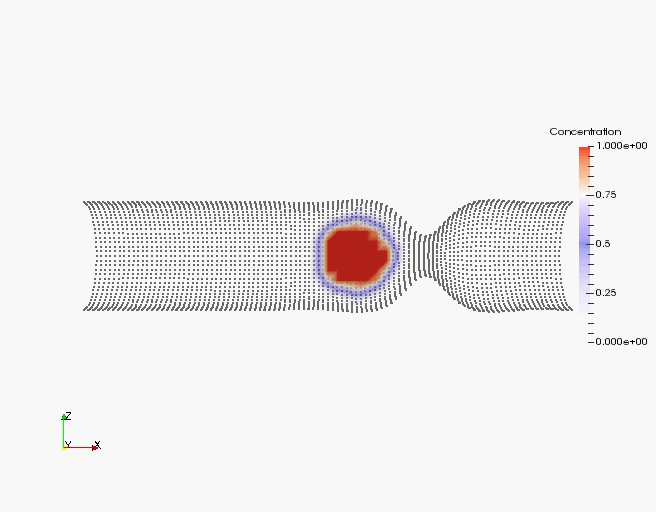
\includegraphics [width=0.45\textwidth] {strong_stenosis_0.png}
  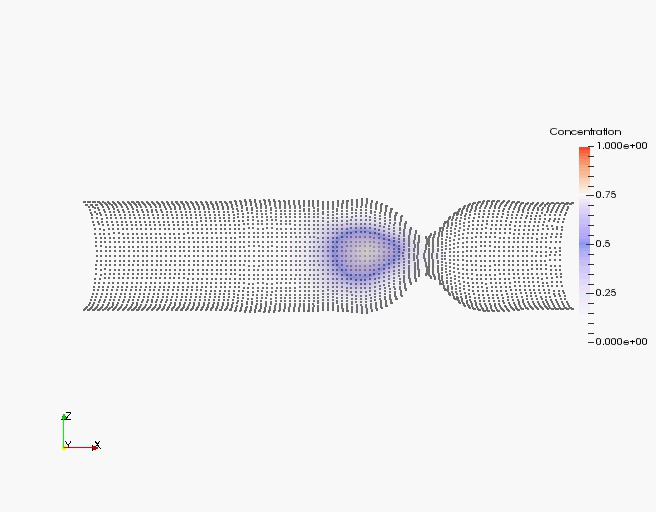
\includegraphics [width=0.45\textwidth] {strong_stenosis_1.png}
  \caption{Динамика движения тромба при наличии стеноза сильной степени}
  \label{img:strong_stenosis}
\end{figure}

\textbf{Третья глава} содержит три параграфа и посвящена решению задачи о
движении лепестков искусственного сердечного клапана под воздействием давления
вязкой несжимаемой неоднородной жидкости, a также верификации описанной модели.
Приводятся результаты расчетов работы клапана, их сравнение с
экспериментальными данными, а также сравнение с результатами, полученными в
других работах.  Постановка задачи аналогична описанной в \textbf{главе 1}.
Т.к. в данном случае объектом исследования является клапан, стенки сосуда являются
абсолютно жесткими. Схема расположения клапана изображена на Рис. \ref{img:aorta_boundaries}

\begin{figure}[h]
  \center
  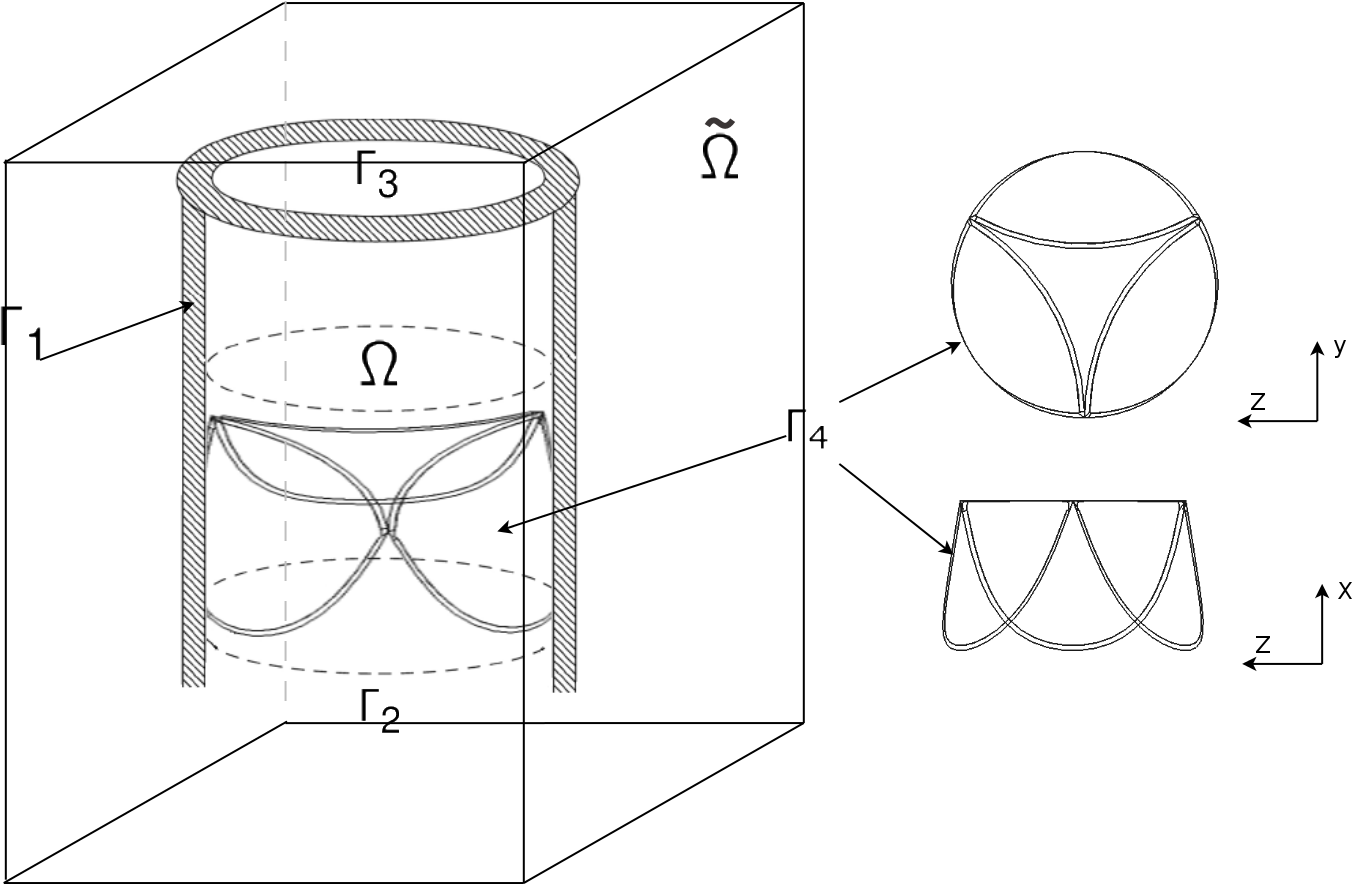
\includegraphics [width=0.8\textwidth] {aorta_valve_scheme_flat_computation.png}
  \caption{Изображение границ расчетной области}
  \label{img:aorta_boundaries}
\end{figure}

В \textbf{параграфе 3.1} представлены результаты решения задачи о динамике
искусственного сердечного клапана для случая однородной и неоднородной жидкости.
На Рис. \ref{img:ideal_valve_dynamics} показана динамика движения лепестков клапана
с жесткостью $k_s=5 \cdot 10^3, k_b=5 \cdot 10^{3}$ под воздействием перепада
давления $\triangle P = 6$ однородной жидкости $\mu = 0.01, \rho=1$.

\begin{figure}[H]
  \center
  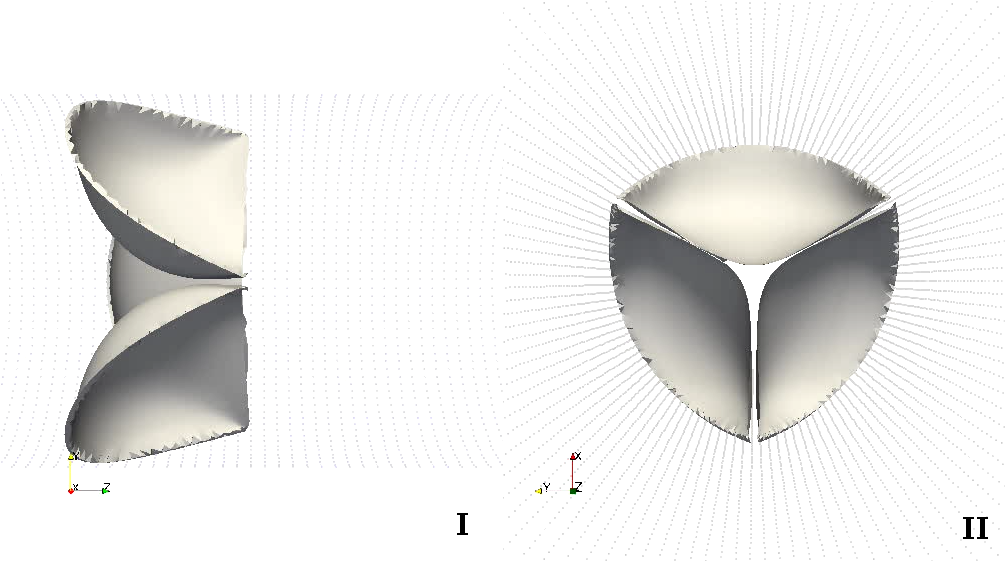
\includegraphics [width=0.45\textwidth] {valve_1.png}
  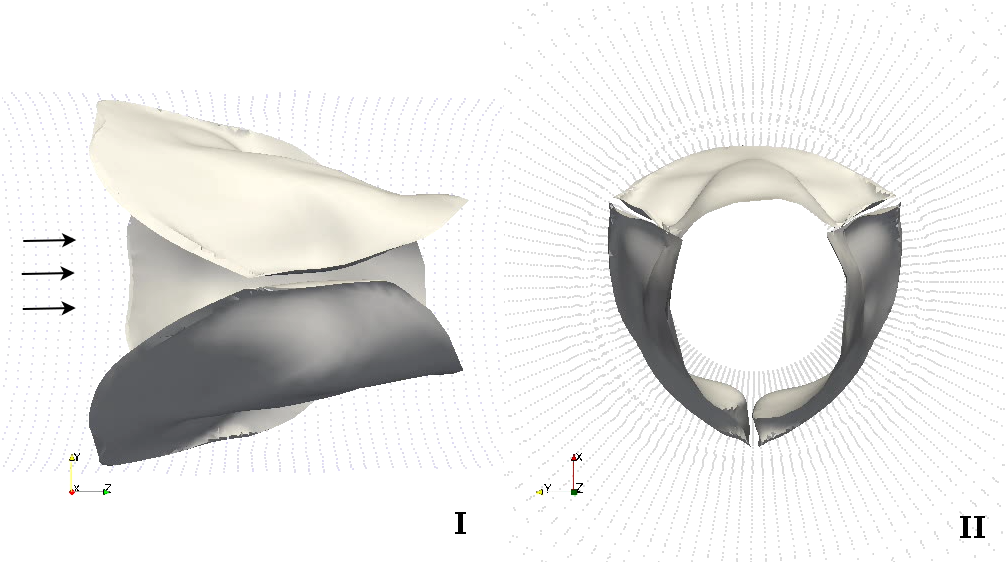
\includegraphics [width=0.45\textwidth] {valve_2.png}
  \caption{Динамика деформации лепестков клапана в начальный момент времени, и в момент наибольшего раскрытия}
  \label{img:ideal_valve_dynamics}
\end{figure}

Т.к. характеристики потока жидкости имеют непосредственное влияние на динамику клапана,
были провередены расчеты, демонстрирующие распределение примеси в сосуде
после нескольких циклов работы клапана. В начальный момент времени сосуд равномерно заполнен
примесью, которая составляет 45\% от общего объема и имеет параметры $\rho_1 = 1.2, \mu_1=0.02$.
Итоговое распределение примеси после трех циклов работы клапана имеет пульсовый характер
и представлено на Рис. \ref{img:admixture_distribution}).

\begin{figure}[H]
  \center
  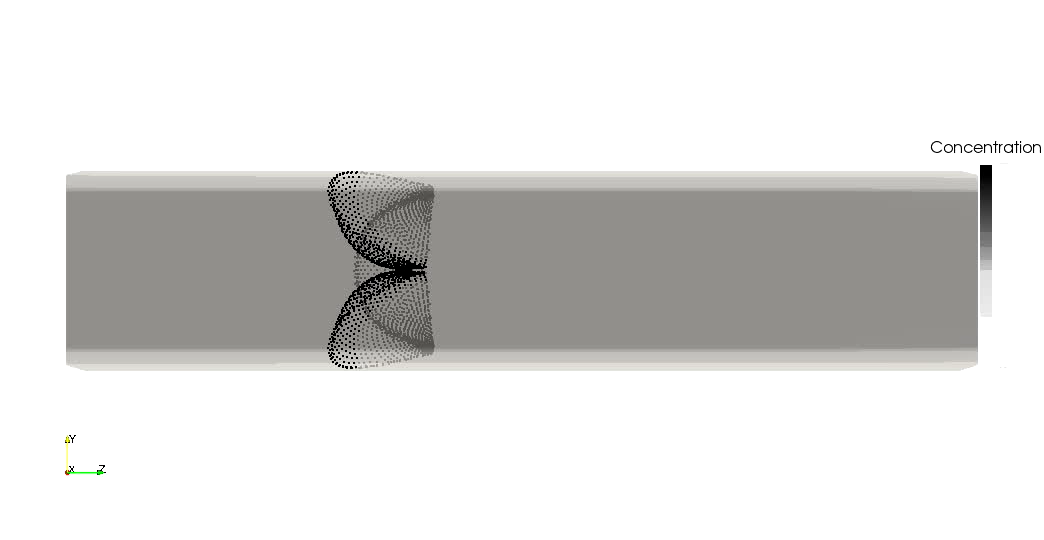
\includegraphics [width=0.45\textwidth] {valve_in_mixture1.png}
  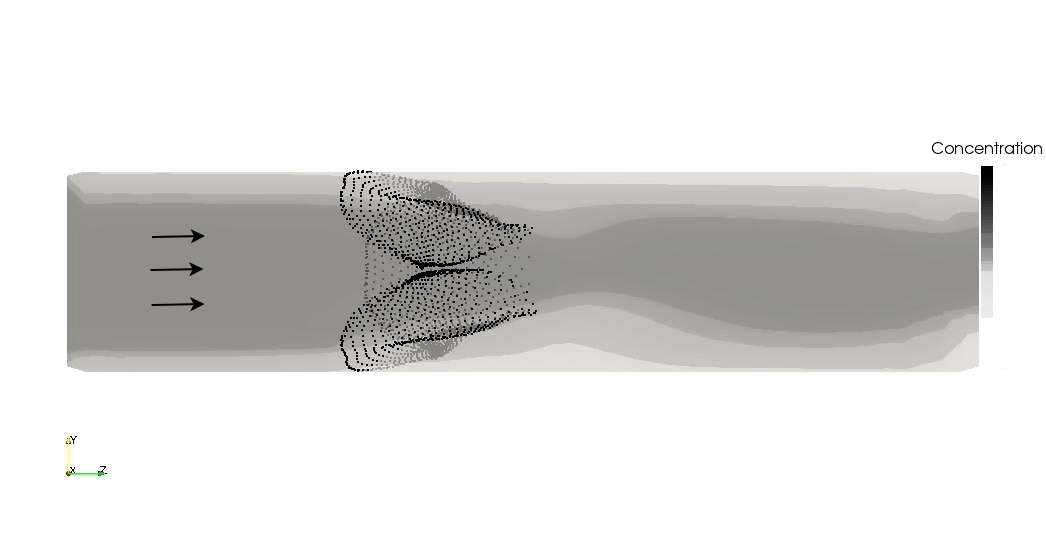
\includegraphics [width=0.45\textwidth] {valve_in_mixture2.png}
  \caption{Распределение примеси в сосуда после трех циклов работы клапана}
  \label{img:admixture_distribution}
\end{figure}

В \textbf{параграфе 3.2} описаны результаты решения задачи динамике
искусственного сердечного клапана <<Юнилайн>> для случая однородной и
неоднородной жидкости. Приведены сравнения полученных результатов с экспериментальными данными,
а также с результатами других авторов.

Моделирование клапана <<Юнилайн>> отличается более реалистичной геометрией лепестков а также наличием
фиброзного кольца и гибких стоек, к которым крепятся лепески. На Рис. \ref{img:uniline}
приведена динамика клапана с жесткостью $k_s=8 \cdot 10^{3}, k_b=2.5 \cdot 10^{3}$ в потоке
набегающей жидкости с параметрами $\rho = 1, \mu = 0.01$ и перепадом давления $\triangle P = 7$.

%\begin{wrapfigure}{L}{0.5\textwidth}
\begin{figure}{H}
  \center
  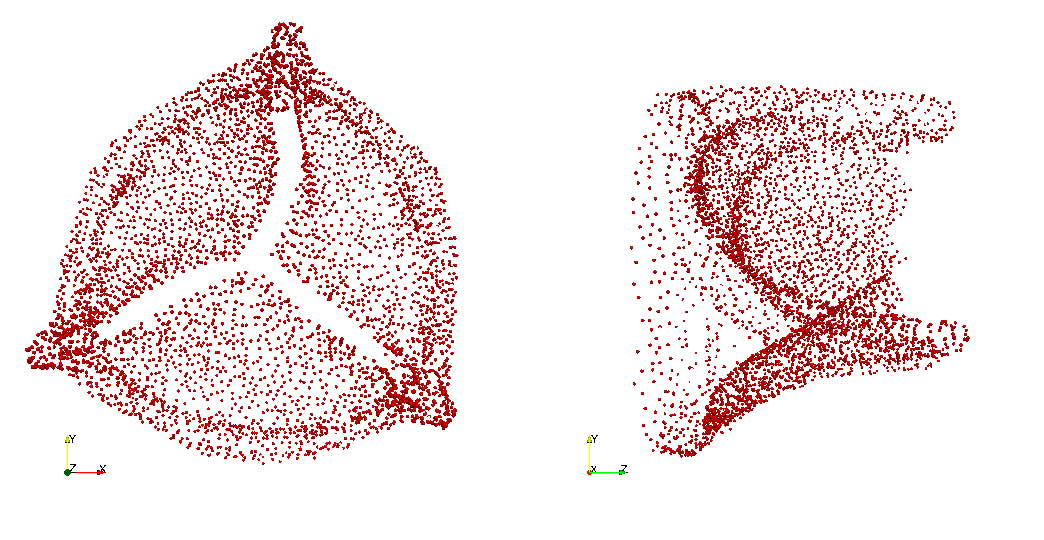
\includegraphics [width=0.5\textwidth] {real_valve1_1.png}
  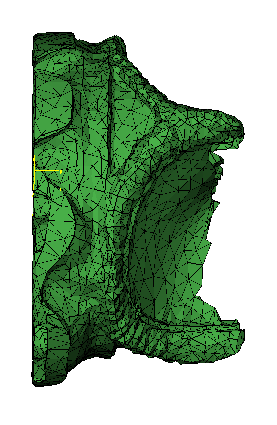
\includegraphics [width=0.5\textwidth] {real_valve2_1.png}
  \caption{Динамика работы клапана <<Юнилайн>>}
  \label{img:uniline}
\end{figure}
%\end{wrapfigure}

Для верификации модели было проведено сравнение результатов расчета в размерных переменных расхода жидкости
с аналогичными данными из работы Griffith B.E.\footnote{Griffith B.E., Immersed boundary model of aortic heart
valve dynamics with physiological driving and loading conditions. // Int J Numer Meth Biomed Eng, 28:317-345, 2012}
\begin{figure}[H]
  \center
  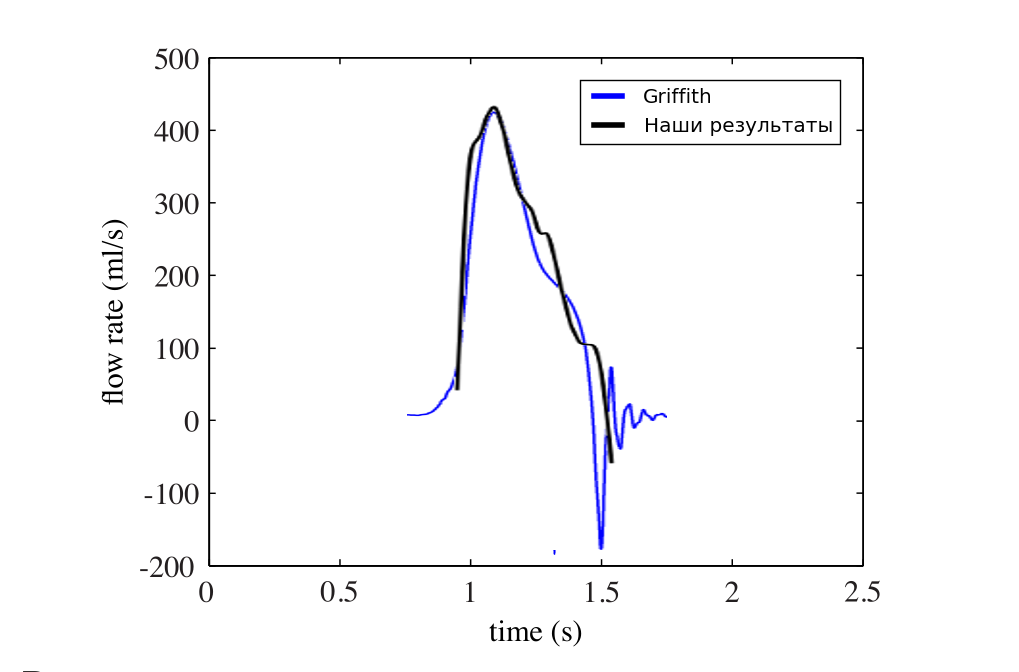
\includegraphics [width=0.8\textwidth] {flow_rate_comparison_with_legend.png}
  \caption{Графики расхода жидкости в проведенных расчетах с данными других авторов}
  \label{img:flow_rate_griffith}
\end{figure}

На Рис. \ref{img:flow_rate_griffith} показаны результаты сравнения. Расчеты
были проведены для реальных параметров крови и физиологичного давления.
Сравнение демонстрирует достаточно хороший уровень совпадения, несмотря на
некоторые отличия (например, наличие фиброзного кольца в наших расчетах, или
отсутствие синусов вальсальвы).

Помимо этого было проведено сравнение с экспериментальными данными, полученными
на стенде Pulse Duplicator System от Vivitro Labs на базе ФГБУ НИИ КПССЗ СО РАМН, г. Кемерово.
На Рис. \ref{img:flow_rate_experiment} показаны результаты сравнения, где видно, что расход достаточно хорошо
совпадает в фазах открытия и закрытия клапана, но графики различаются в фазе полного раскрытия.

\begin{figure}[H]
  \center
  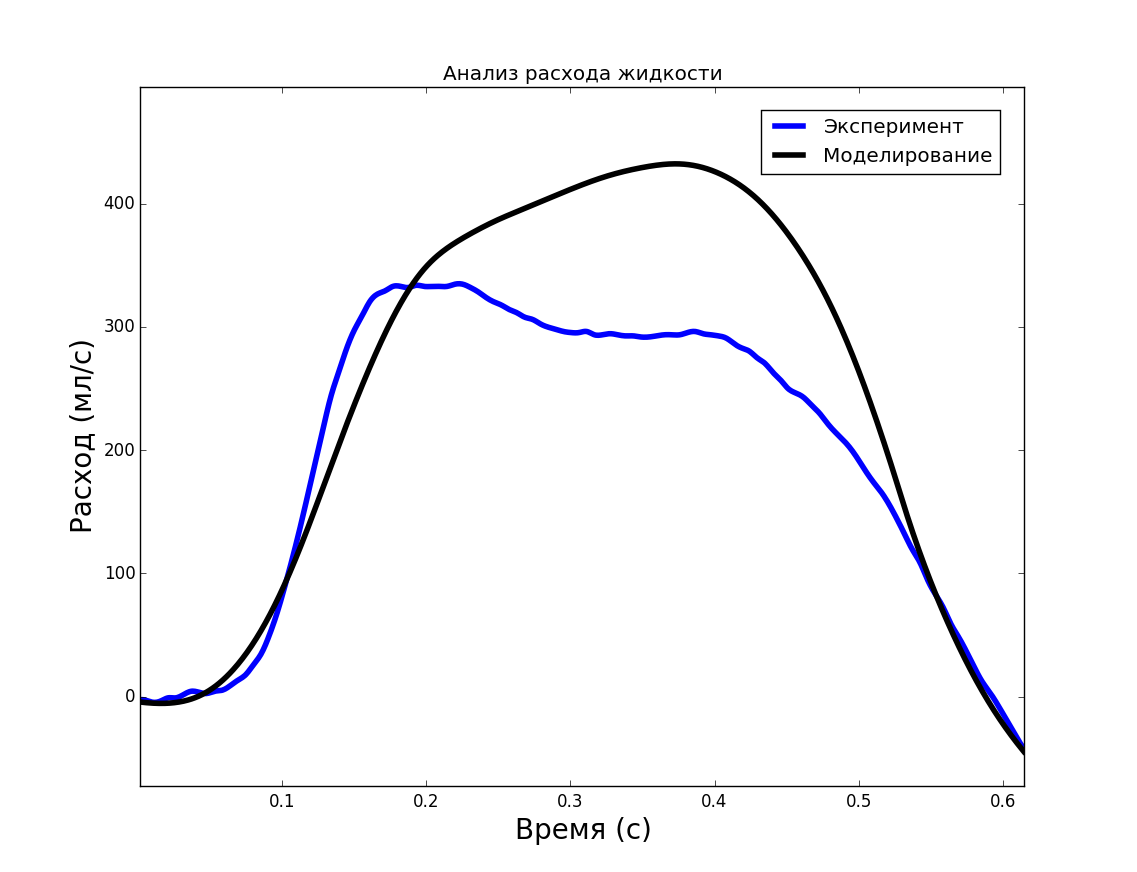
\includegraphics [width=0.6\textwidth] {flowrate_experiment_with_legend.png}
  \caption{Графики расхода жидкости в проведенных расчетах с экспериментальными данными}
  \label{img:flow_rate_experiment}
\end{figure}

В \textbf{параграфе 3.3} приведены результаты исследования зависимости
распределения напряжения по поверхности искусственного клапана <<Юнилайн>>
в зависимости от параметров жидкости и наличия примесей в ней. Этот аспект часто
игнорируется в научных работах, однако как показано в работе, он достаточно важен.
На Рис. \ref{img:force_distribution} приведены графики напряжения в некоторых характерных
точках клапана для случаев его работы в однородной и неоднородной жидкости.

\begin{figure}[H]
  \center
  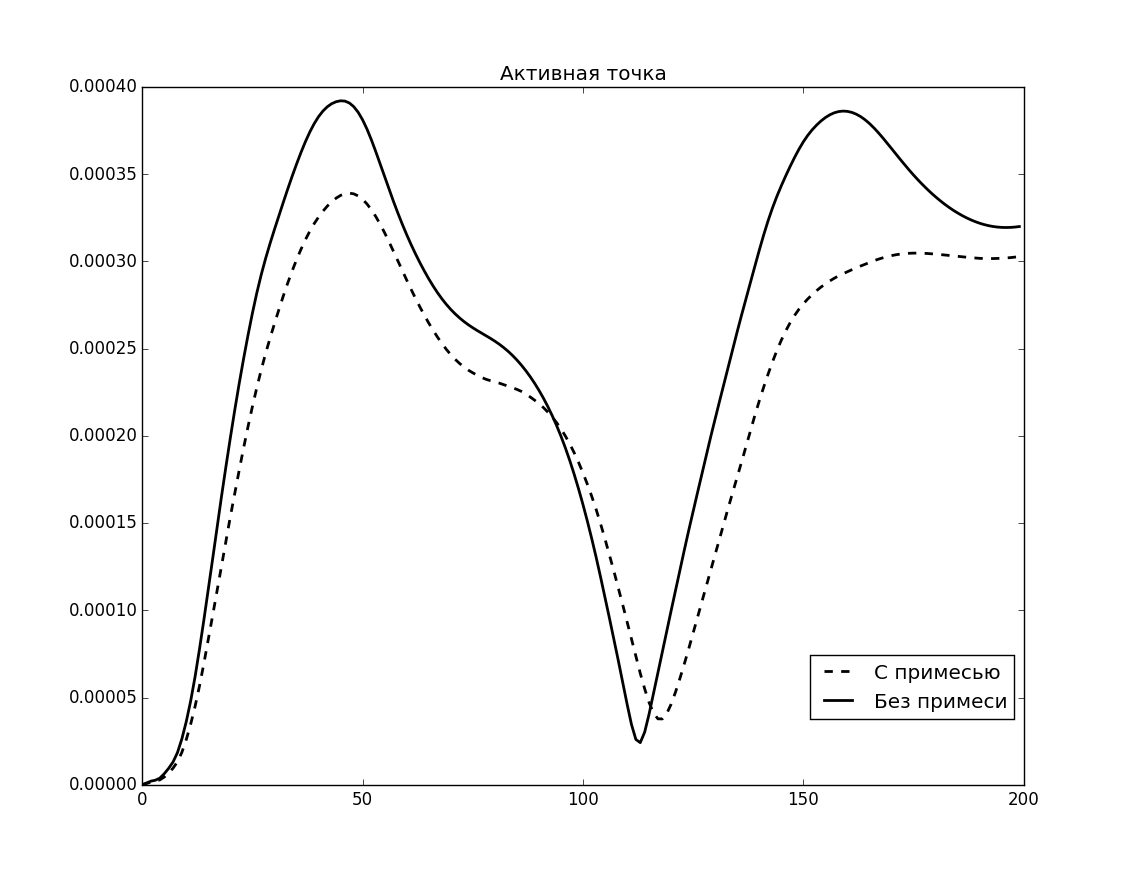
\includegraphics [width=0.45\textwidth] {forces_active_point.png}
  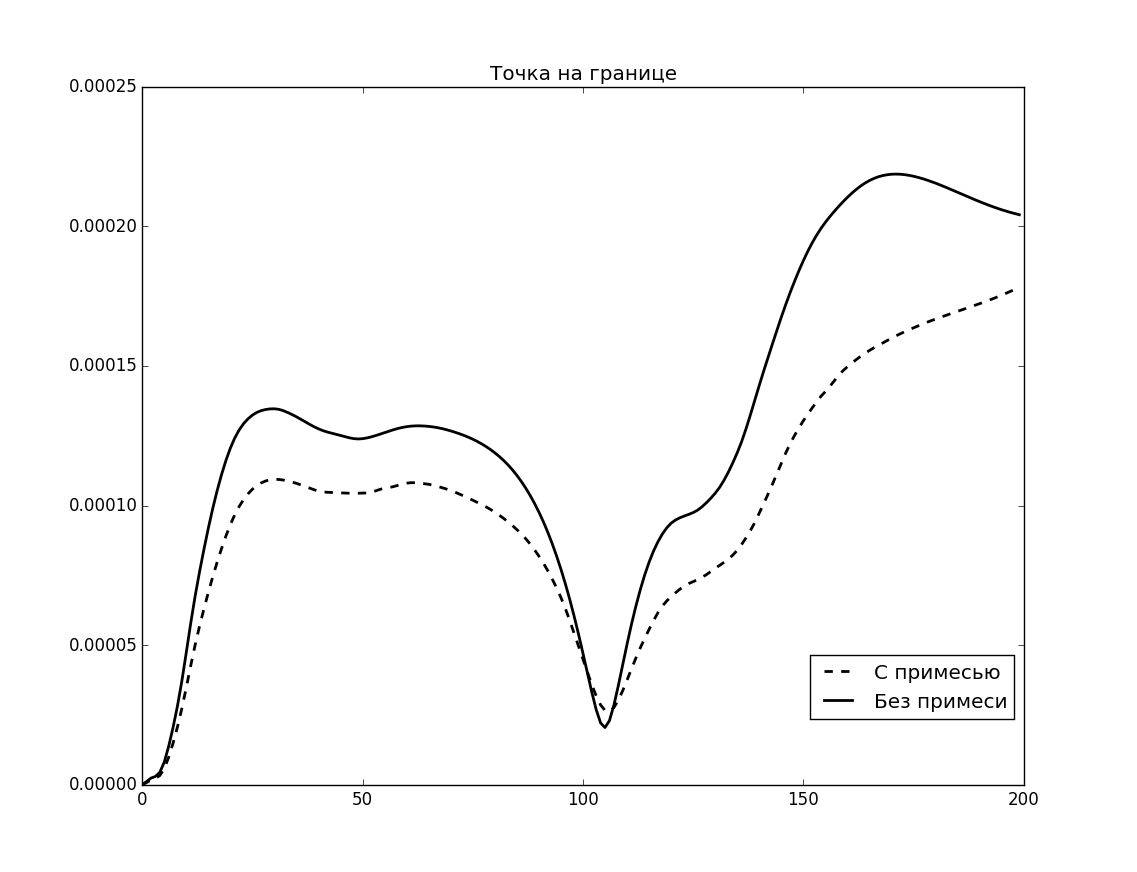
\includegraphics [width=0.45\textwidth] {forces_boundary_point.png}
  \caption{Напряжение на характерных точках клапана для расчетов без примеси и с ее наличием в сосуде}
  \label{img:force_distribution}
\end{figure}

Как видно из графиков, наличие примеси снижает напряжение, делая его перепады меньше и внося небольшое
смещение по времени относительно циклов работы клапана. Это показыват, что факт наличия неоднородностей
любого характера в крови может серьезно влиять на работу клапана.\\

В \textbf{заключении} приводятся основные результаты работы:
\begin{enumerate}
 \item Предложенный в работе подход позволяет успешно решать трехмерные задачи
     о теении вязкой неоднородной несжимаемой жидкости в сосудах с
     деформируемыми стенками и тонкими гибкими препятствиями
 \item Разработанный программный комплекс может применяться для моделирования
     широкого круга задач, связанных с работой сердечного клапана и течением
     крови в сосудах
 \item Наличие примеси в жидкости непосредственно влияет на напряжения, возникаюшие
     при деформации створок и фиброзного кольца искусственного клапана
\end{enumerate}

%\newpage
\renewcommand{\refname}{\Large Публикации автора по теме диссертации}
\nocite{*}
\bibliography{biblio}
